
\section{Anhang}



%%%
%%% SCENARIO Seq
%%%

\begin{frame}
  \frametitle{Szenario Client\,/\,Server}
  \begin{block}{Einstellungen}
    \begin{itemize}  
      \item 1 Super-Peer und 63 Peers
      \vspace{2mm}
      \item Peers sind untereinander nicht verbunden
      \vspace{2mm}
      \item Anzahl der Chunks spielt keine Rolle
      \vspace{2mm}
      \item Datengröße so gewählt, dass $T_0=10$ Minuten gilt.
    \end{itemize}   
  \end{block}
\end{frame}

\begin{frame}
  \frametitle{Szenario Client\,/\,Server - Completion}
  \begin{itemize}  
    \item Links: Ablauf des Datentransfers
    \item Rechts: Peers absteigend sortiert nach Gesamtdauer
  \end{itemize}

  \begin{center}
    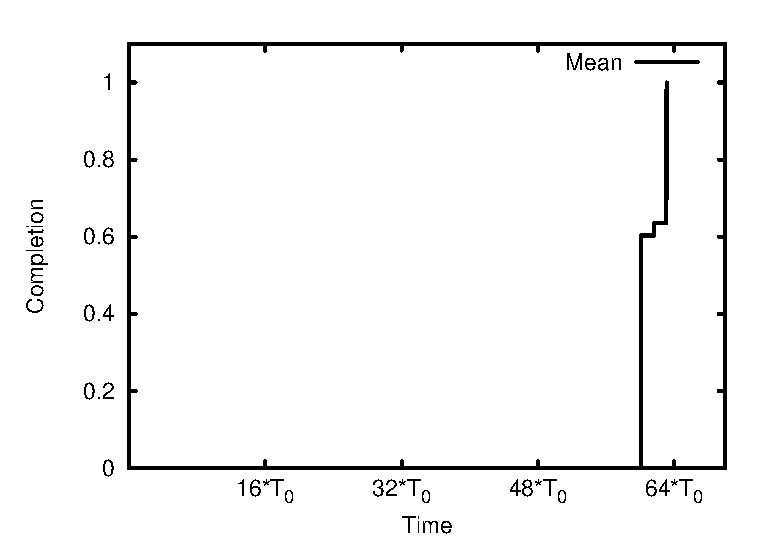
\includegraphics[width=0.49\textwidth]{fig/plots/scenario_2_seq/plots/GeneratedMeanChunkCompletion.csv.eps}
    \hfill
    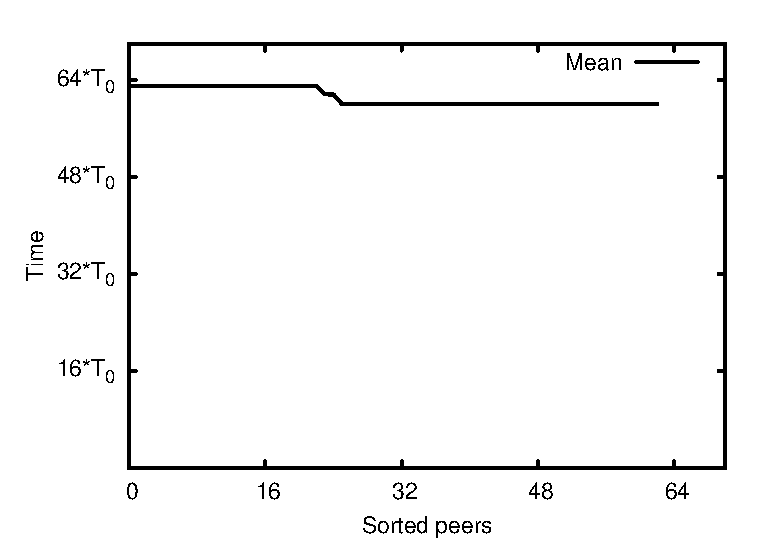
\includegraphics[width=0.49\textwidth]{fig/plots/scenario_2_seq/plots/GeneratedMeanSortedChunkCompletion.csv.eps}
  \end{center}
\end{frame}


\begin{frame}
  \frametitle{Szenario Client\,/\,Server - Upload/Download}
    \begin{itemize}  
    \item Links: Uploadbandbreite des Super-Peers
    \item Rechts: Downloadbandbreite der Peers
  \end{itemize}
  \begin{center}
    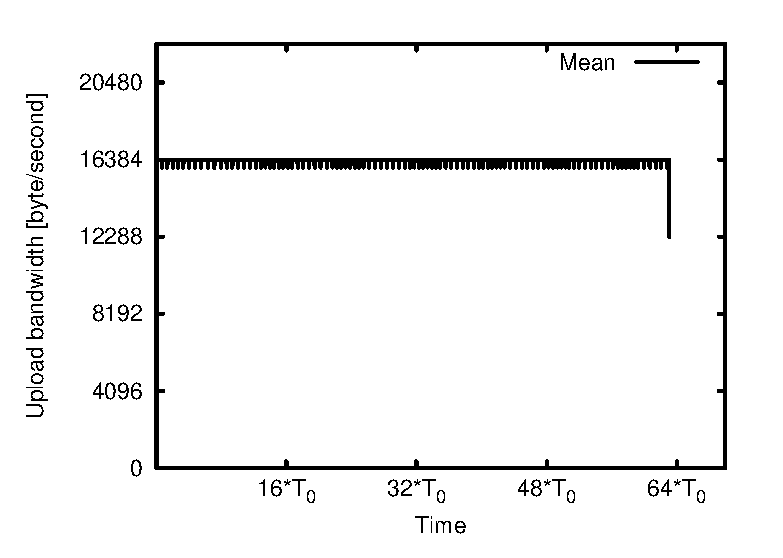
\includegraphics[width=0.49\textwidth]{fig/plots/scenario_2_seq/plots/GeneratedMeanCurrentSuperSeederUploadBandwidth.csv.eps}
    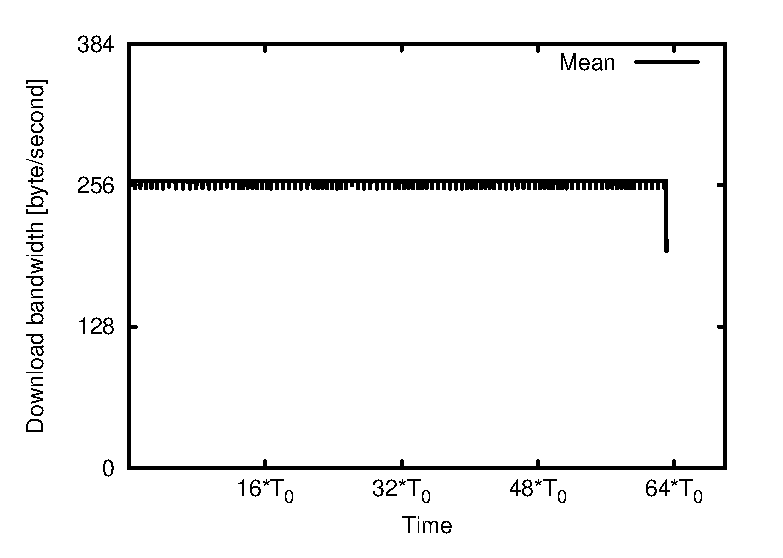
\includegraphics[width=0.49\textwidth]{fig/plots/scenario_2_seq/plots/GeneratedMeanCurrentDownloadBandwidth.csv.eps}
  \end{center}
\end{frame}


%%%
%%% Szenario Log
%%%

\begin{frame}
  \frametitle{Szenario Logarithmic}
  \begin{block}{Einstellungen}
    \begin{itemize}  
      \item 1 Super-Peer und 63 Peers
      \vspace{2mm}
      \item Peers (auch Super-Peer) senden gleichzeitig an max. einen Peer
      \vspace{2mm}
      \item Datensatz wird vollständig übertragen (kein Chunking)
      \vspace{2mm}
      \item Anzahl sendender Peers wächst exponentiell
      \vspace{2mm}
      \item Datengröße so gewählt, dass $T_0=10$ Minuten gilt.
    \end{itemize}   
  \end{block}
\end{frame}

\begin{frame}
  \frametitle{Szenario Logarithmic - Completion}
  \begin{itemize}  
    \item Links: Ablauf des Datentransfers
    \item Rechts: Peers absteigend sortiert nach Gesamtdauer
  \end{itemize}

  \begin{center}
    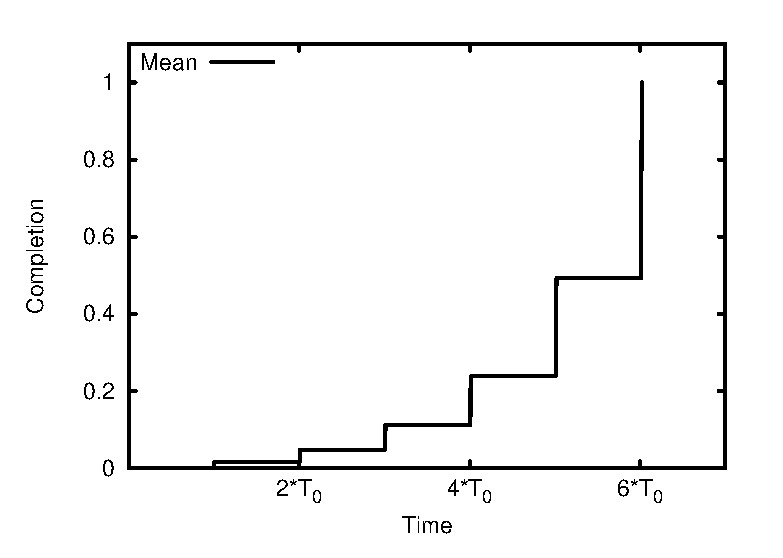
\includegraphics[width=0.49\textwidth]{fig/plots/scenario_3_log/plots/GeneratedMeanChunkCompletion.csv.eps}
    \hfill
    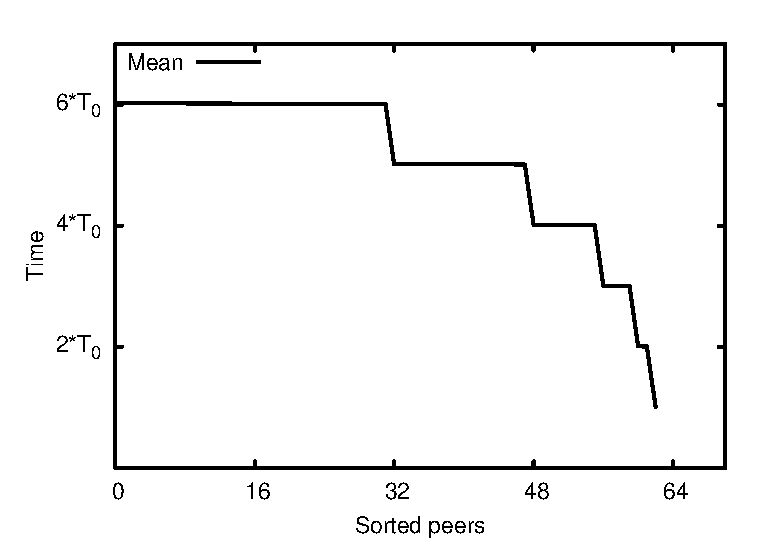
\includegraphics[width=0.49\textwidth]{fig/plots/scenario_3_log/plots/GeneratedMeanSortedChunkCompletion.csv.eps}
  \end{center}
\end{frame}


\begin{frame}
  \frametitle{Szenario Logarithmic - Upload/Download}
  \begin{center}
    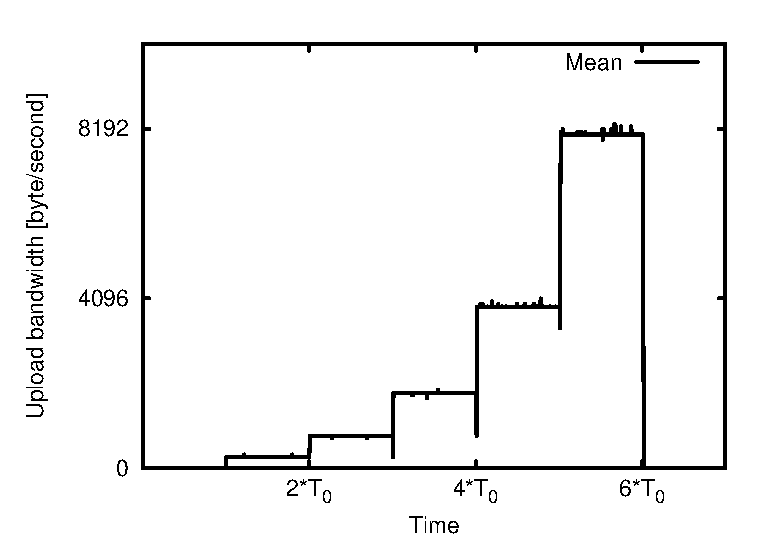
\includegraphics[width=0.49\textwidth]{fig/plots/scenario_3_log/plots/GeneratedMeanCurrentUploadBandwidth.csv.eps}
    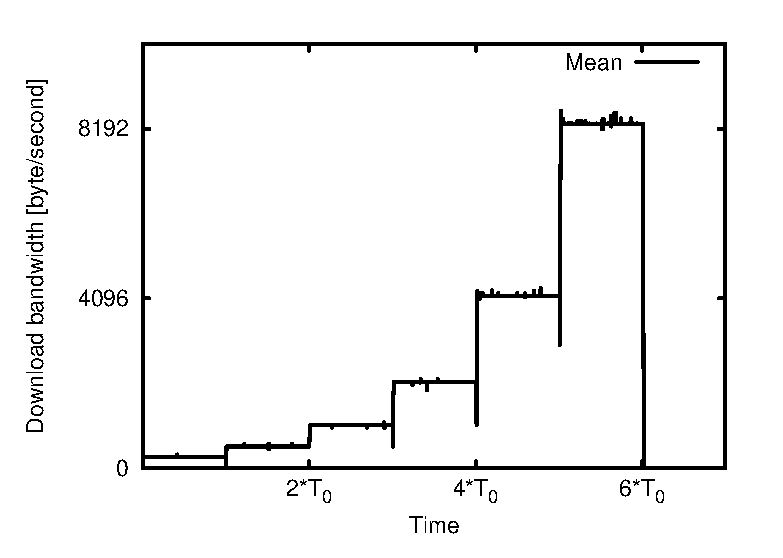
\includegraphics[width=0.49\textwidth]{fig/plots/scenario_3_log/plots/GeneratedMeanCurrentDownloadBandwidth.csv.eps}
  \end{center}
\end{frame}


\begin{frame}
  \frametitle{Szenario Logarithmic - Super-Peer Upload}
  \begin{center}
    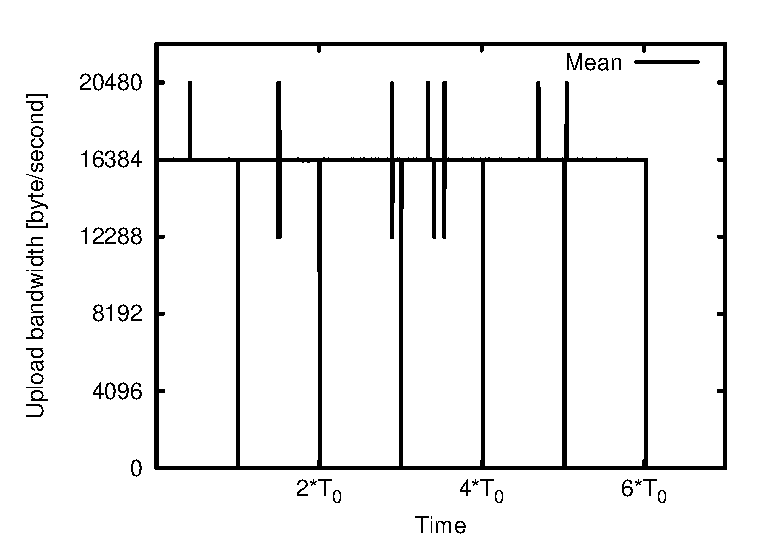
\includegraphics[width=0.49\textwidth]{fig/plots/scenario_3_log/plots/GeneratedMeanCurrentSuperSeederUploadBandwidth.csv.eps}
  \end{center}
\end{frame}


%%%
%%% SCENARIO 192
%%%

\begin{frame}
  \frametitle{Default Szenario mit 192 Peers - Completion}
  \begin{itemize}  
    \item Links: Ablauf des Datentransfers
    \item Rechts: Peers absteigend sortiert nach Gesamtdauer
  \end{itemize}

  \begin{center}
    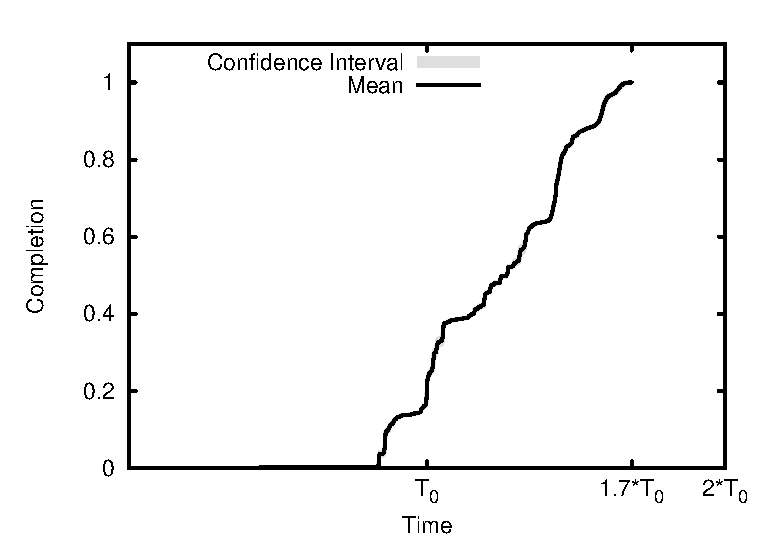
\includegraphics[width=0.49\textwidth]{fig/plots/scenario_11_peer_count_192_v2/plots/GeneratedMeanChunkCompletion.csv.eps}
    \hfill
    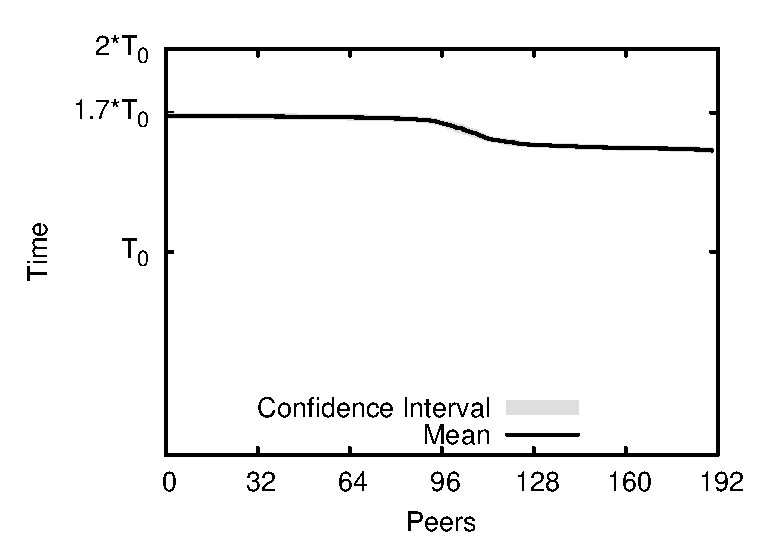
\includegraphics[width=0.49\textwidth]{fig/plots/scenario_11_peer_count_192_v2/plots/GeneratedMeanSortedChunkCompletion.csv.eps}
  \end{center}
\end{frame}


\begin{frame}
  \frametitle{Default Szenario mit 192 Peers - Upload/Download}
  \begin{center}
    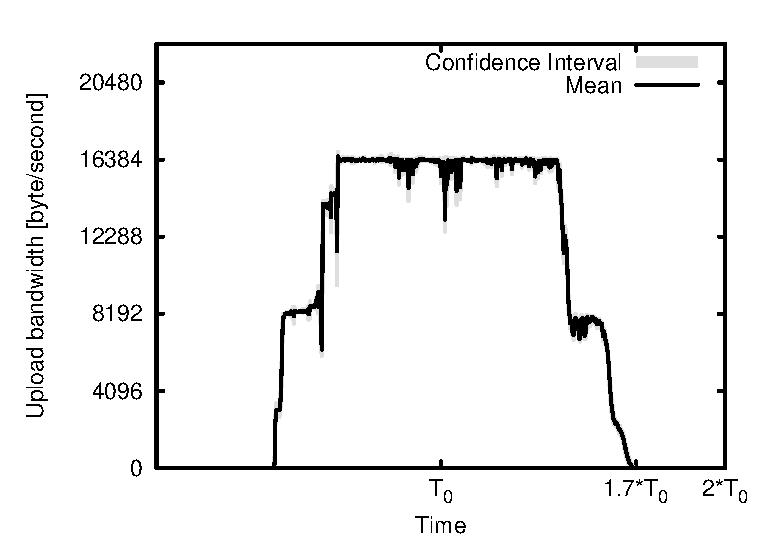
\includegraphics[width=0.49\textwidth]{fig/plots/scenario_11_peer_count_192_v2/plots/GeneratedMeanCurrentUploadBandwidth.csv.eps}
    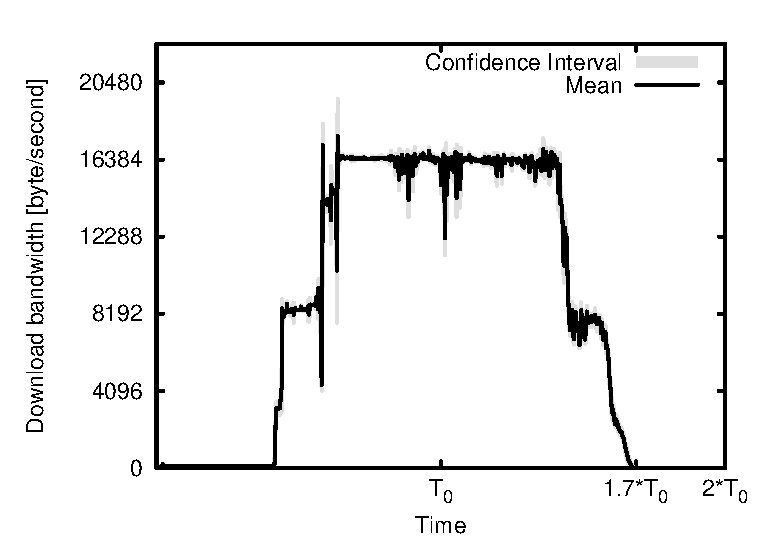
\includegraphics[width=0.49\textwidth]{fig/plots/scenario_11_peer_count_192_v2/plots/GeneratedMeanCurrentDownloadBandwidth.csv.eps}
  \end{center}
\end{frame}


\begin{frame}
  \frametitle{Default Szenario mit 192 Peers - Super-Peer Upload}
  \begin{center}
    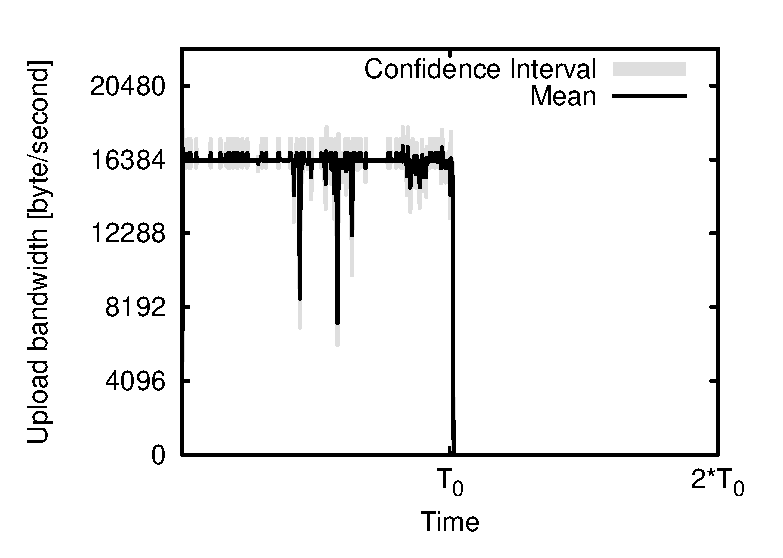
\includegraphics[width=0.49\textwidth]{fig/plots/scenario_11_peer_count_192_v2/plots/GeneratedMeanCurrentSuperSeederUploadBandwidth.csv.eps}
  \end{center}
\end{frame}


%%%
%%% Szenario MetaData 0
%%%

\begin{frame}
  \frametitle{Default Szenario mit Meta-Daten 0 - Completion}
  \begin{itemize}  
    \item Links: Ablauf des Datentransfers
    \item Rechts: Peers absteigend sortiert nach Gesamtdauer
  \end{itemize}

  \begin{center}
    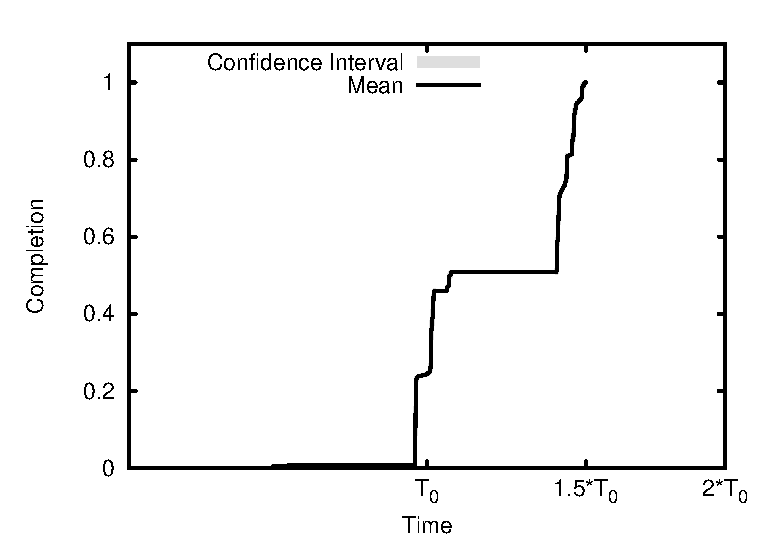
\includegraphics[width=0.49\textwidth]{fig/plots/scenario_5_meta_data_0/plots/GeneratedMeanChunkCompletion.csv.eps}
    \hfill
    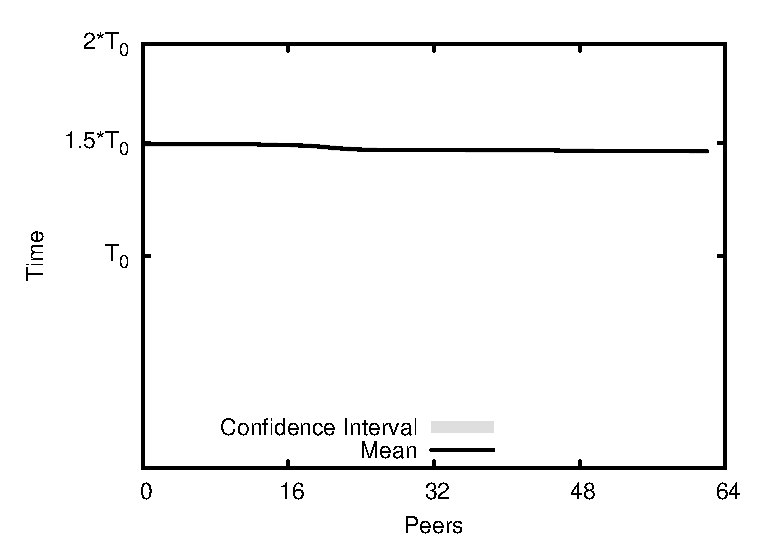
\includegraphics[width=0.49\textwidth]{fig/plots/scenario_5_meta_data_0/plots/GeneratedMeanSortedChunkCompletion.csv.eps}
  \end{center}
\end{frame}


\begin{frame}
  \frametitle{Default Szenario mit Meta-Daten 0 - Upload/Download}
  \begin{center}
    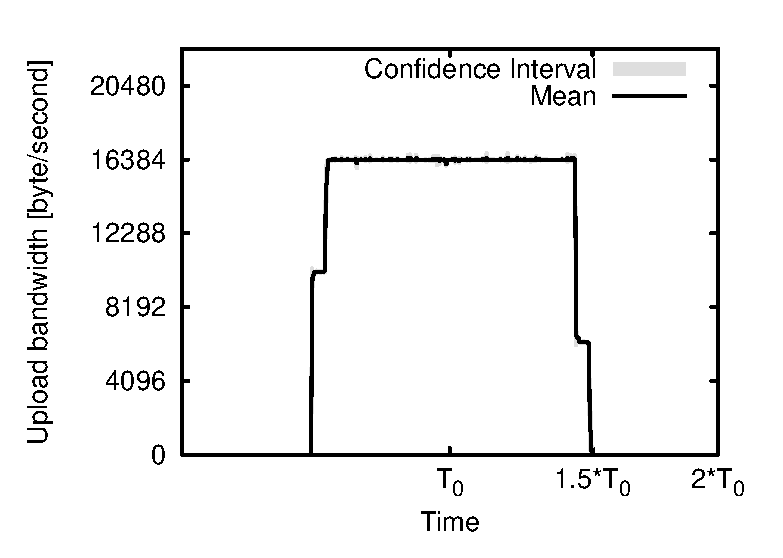
\includegraphics[width=0.49\textwidth]{fig/plots/scenario_5_meta_data_0/plots/GeneratedMeanCurrentUploadBandwidth.csv.eps}
    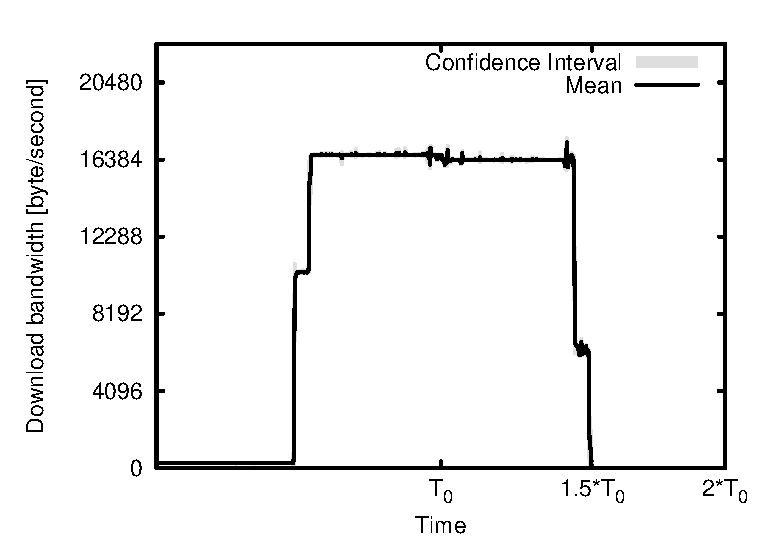
\includegraphics[width=0.49\textwidth]{fig/plots/scenario_5_meta_data_0/plots/GeneratedMeanCurrentDownloadBandwidth.csv.eps}
  \end{center}
\end{frame}


\begin{frame}
  \frametitle{Default Szenario mit Meta-Daten 0 - Super-Peer Upload}
  \begin{center}
    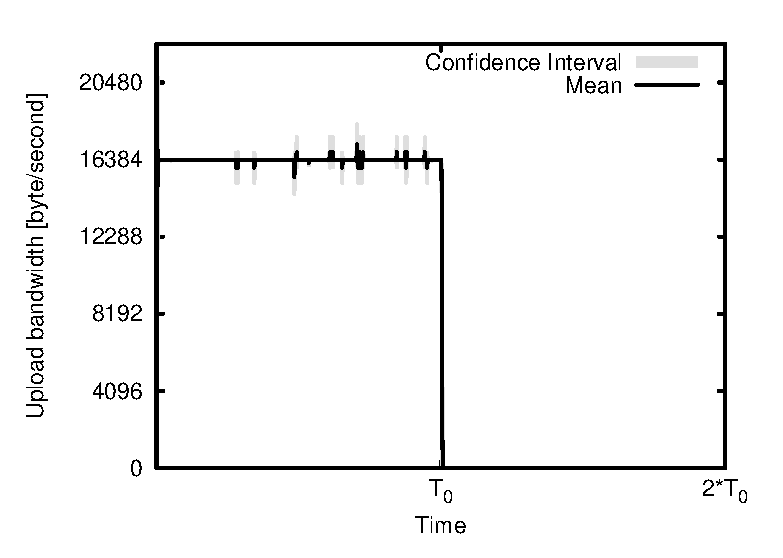
\includegraphics[width=0.49\textwidth]{fig/plots/scenario_5_meta_data_0/plots/GeneratedMeanCurrentSuperSeederUploadBandwidth.csv.eps}
  \end{center}
\end{frame}



%%%
%%% Szenario MetaData 10
%%%

\begin{frame}
  \frametitle{Default Szenario mit Meta-Daten 10 - Completion}
  \begin{itemize}  
    \item Links: Ablauf des Datentransfers
    \item Rechts: Peers absteigend sortiert nach Gesamtdauer
  \end{itemize}

  \begin{center}
    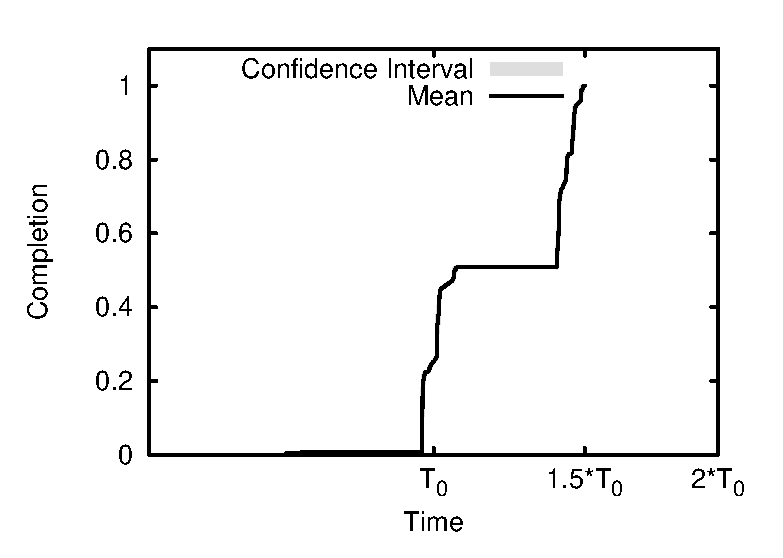
\includegraphics[width=0.49\textwidth]{fig/plots/scenario_10_meta_data_10/plots/GeneratedMeanChunkCompletion.csv.eps}
    \hfill
    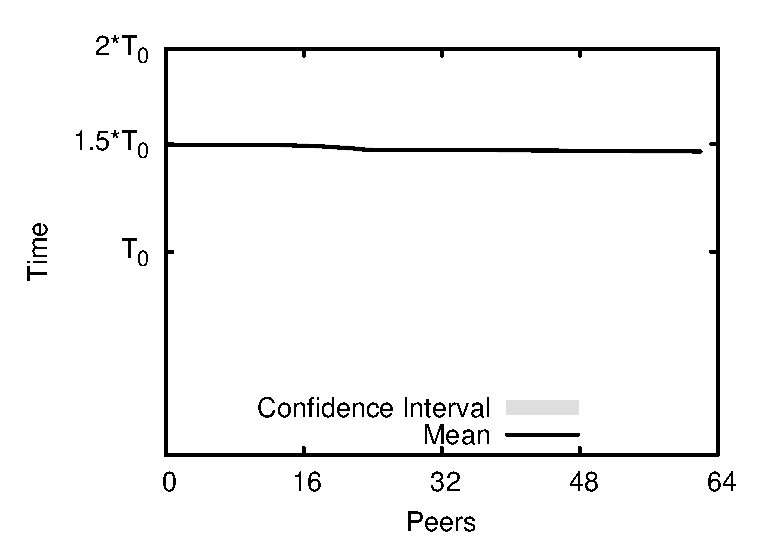
\includegraphics[width=0.49\textwidth]{fig/plots/scenario_10_meta_data_10/plots/GeneratedMeanSortedChunkCompletion.csv.eps}
  \end{center}
\end{frame}


\begin{frame}
  \frametitle{Default Szenario mit Meta-Daten 10 - Upload/Download}
  \begin{center}
    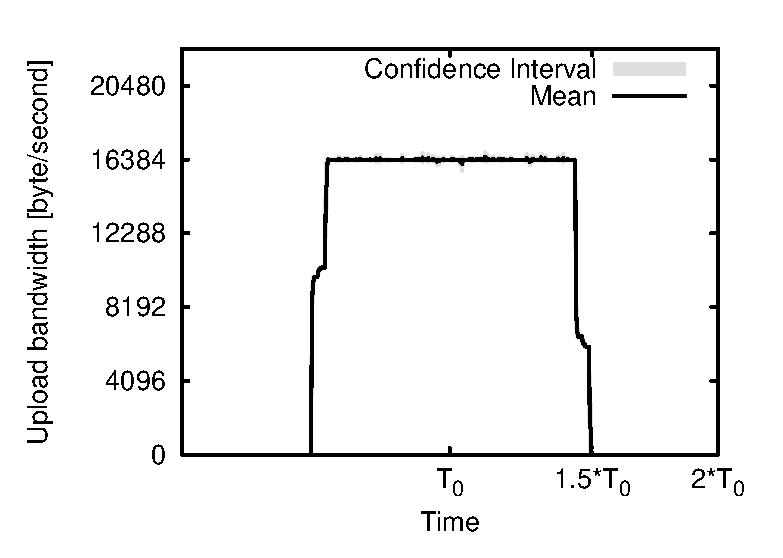
\includegraphics[width=0.49\textwidth]{fig/plots/scenario_10_meta_data_10/plots/GeneratedMeanCurrentUploadBandwidth.csv.eps}
    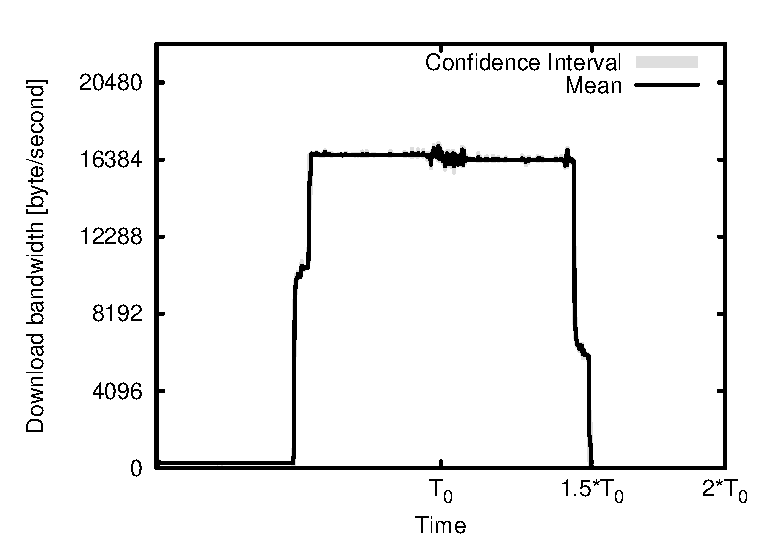
\includegraphics[width=0.49\textwidth]{fig/plots/scenario_10_meta_data_10/plots/GeneratedMeanCurrentDownloadBandwidth.csv.eps}
  \end{center}
\end{frame}


\begin{frame}
  \frametitle{Default Szenario mit Meta-Daten 10 - Super-Peer Upload}
  \begin{center}
    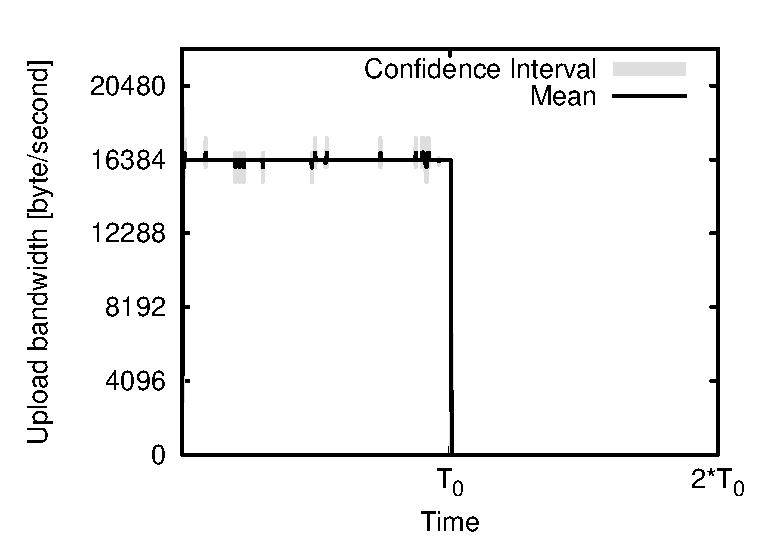
\includegraphics[width=0.49\textwidth]{fig/plots/scenario_10_meta_data_10/plots/GeneratedMeanCurrentSuperSeederUploadBandwidth.csv.eps}
  \end{center}
\end{frame}

%%%
%%% Szenario ChunkFac 1
%%%

\begin{frame}
  \frametitle{Default Szenario mit 1x Chunkanzahl - Completion}
  \begin{itemize}  
    \item Links: Ablauf des Datentransfers
    \item Rechts: Peers absteigend sortiert nach Gesamtdauer
  \end{itemize}

  \begin{center}
    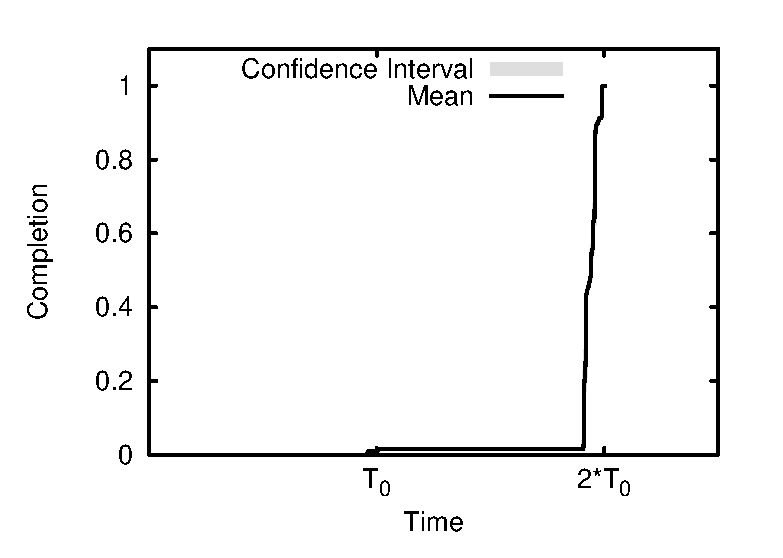
\includegraphics[width=0.49\textwidth]{fig/plots/scenario_7_chunk_count_fac_1/plots/GeneratedMeanChunkCompletion.csv.eps}
    \hfill
    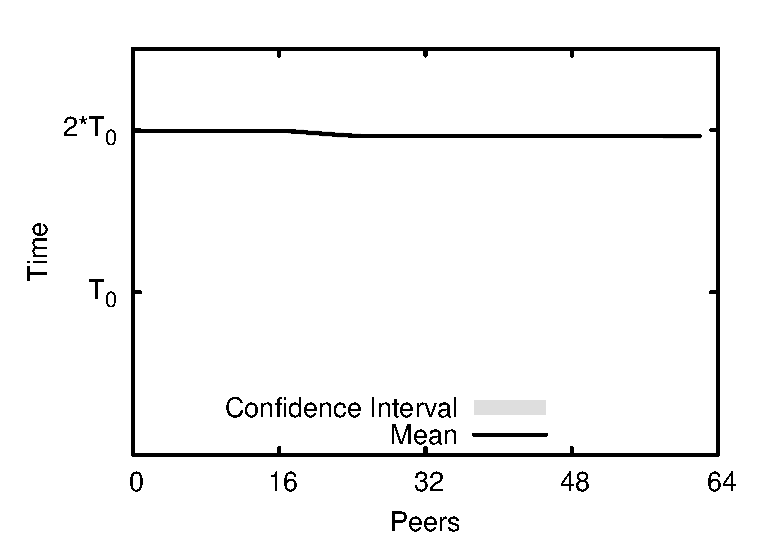
\includegraphics[width=0.49\textwidth]{fig/plots/scenario_7_chunk_count_fac_1/plots/GeneratedMeanSortedChunkCompletion.csv.eps}
  \end{center}
\end{frame}


\begin{frame}
  \frametitle{Default Szenario mit 1x Chunkanzahl - Upload/Download}
  \begin{center}
    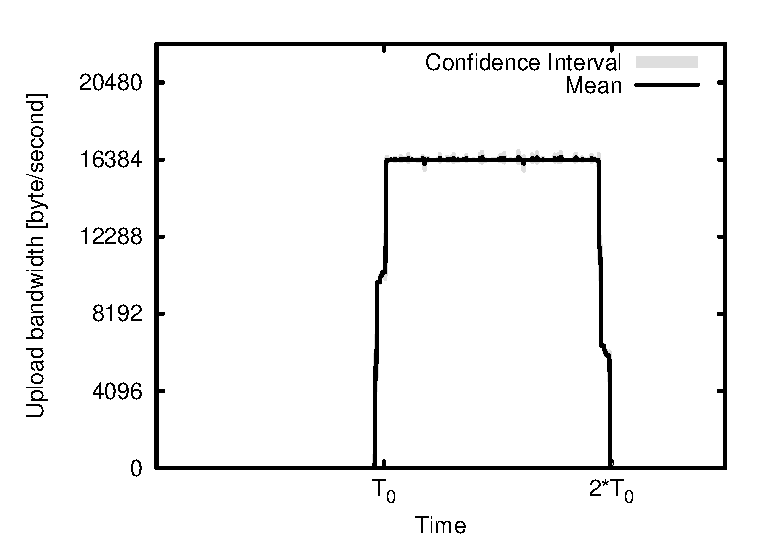
\includegraphics[width=0.49\textwidth]{fig/plots/scenario_7_chunk_count_fac_1/plots/GeneratedMeanCurrentUploadBandwidth.csv.eps}
    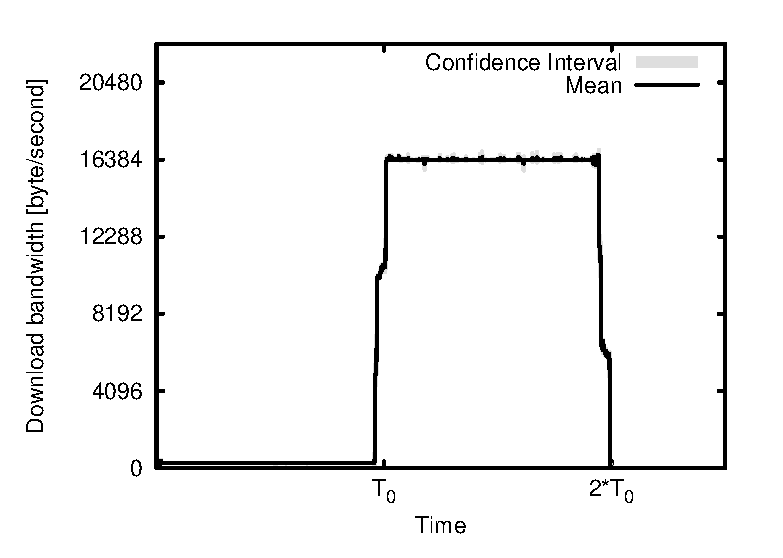
\includegraphics[width=0.49\textwidth]{fig/plots/scenario_7_chunk_count_fac_1/plots/GeneratedMeanCurrentDownloadBandwidth.csv.eps}
  \end{center}
\end{frame}


\begin{frame}
  \frametitle{Default Szenario mit 1x Chunkanzahl - Super-Peer Upload}
  \begin{center}
    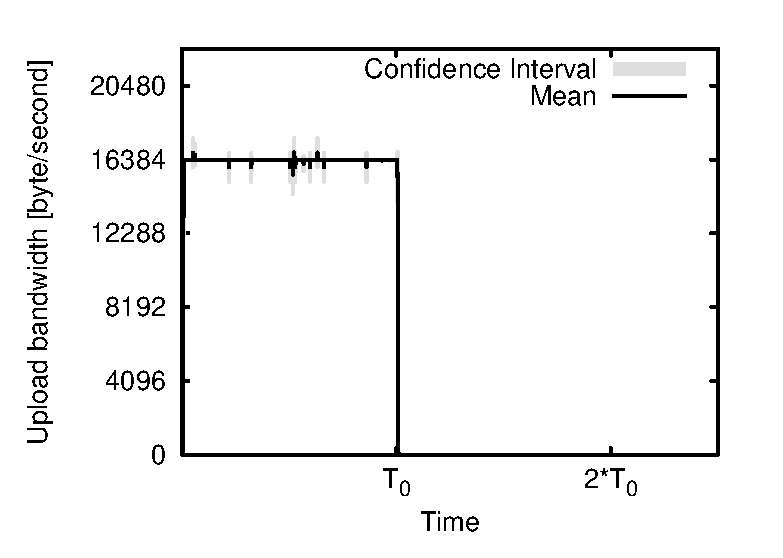
\includegraphics[width=0.49\textwidth]{fig/plots/scenario_7_chunk_count_fac_1/plots/GeneratedMeanCurrentSuperSeederUploadBandwidth.csv.eps}
  \end{center}
\end{frame}

%%%
%%% Szenario ChunkFac 8
%%%

\begin{frame}
  \frametitle{Default Szenario mit 8x Chunkanzahl - Completion}
  \begin{itemize}  
    \item Links: Ablauf des Datentransfers
    \item Rechts: Peers absteigend sortiert nach Gesamtdauer
  \end{itemize}

  \begin{center}
    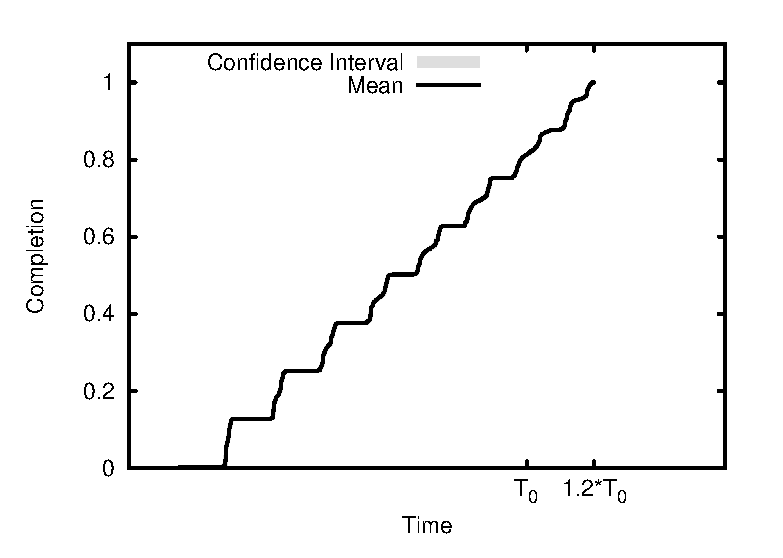
\includegraphics[width=0.49\textwidth]{fig/plots/scenario_16_chunk_count_fac_8/plots/GeneratedMeanChunkCompletion.csv.eps}
    \hfill
    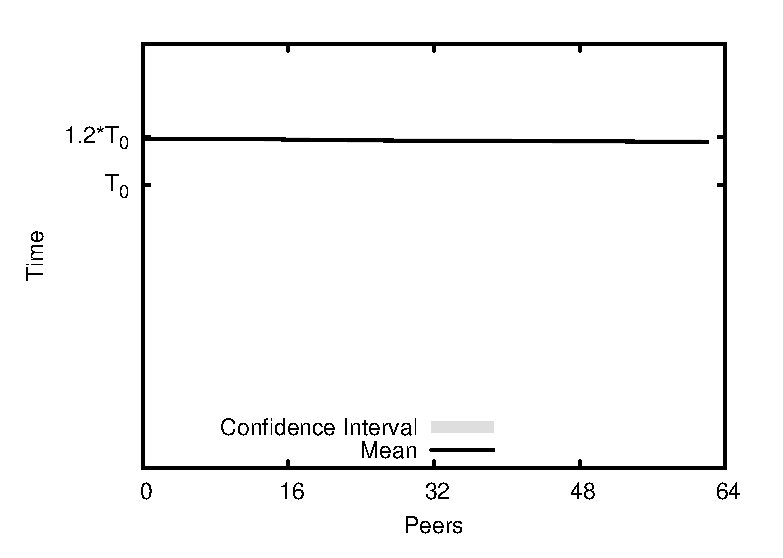
\includegraphics[width=0.49\textwidth]{fig/plots/scenario_16_chunk_count_fac_8/plots/GeneratedMeanSortedChunkCompletion.csv.eps}
  \end{center}
\end{frame}


\begin{frame}
  \frametitle{Default Szenario mit 8x Chunkanzahl - Upload/Download}
  \begin{center}
    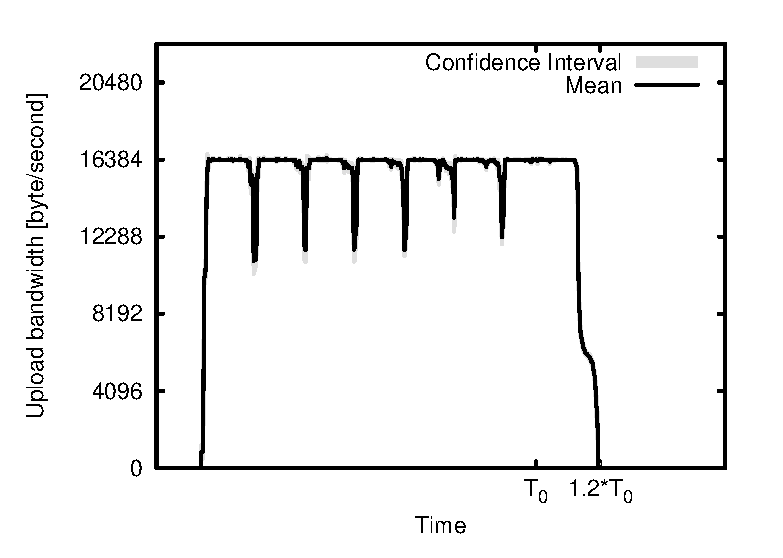
\includegraphics[width=0.49\textwidth]{fig/plots/scenario_16_chunk_count_fac_8/plots/GeneratedMeanCurrentUploadBandwidth.csv.eps}
    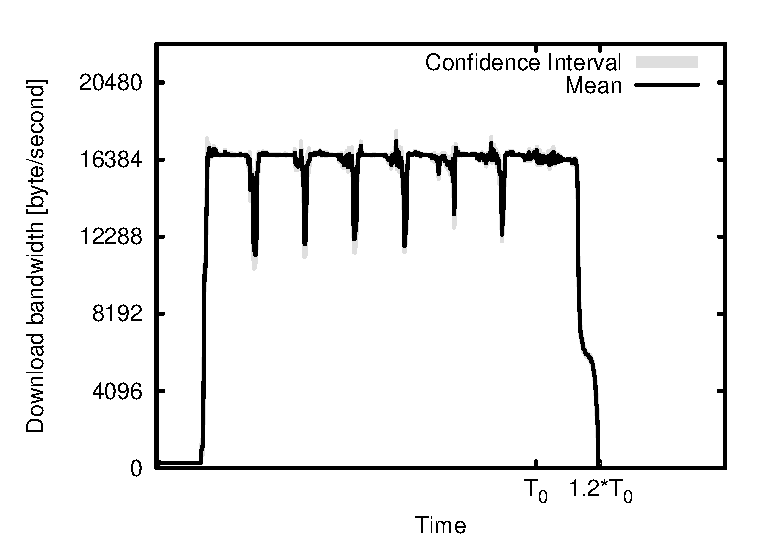
\includegraphics[width=0.49\textwidth]{fig/plots/scenario_16_chunk_count_fac_8/plots/GeneratedMeanCurrentDownloadBandwidth.csv.eps}
  \end{center}
\end{frame}


\begin{frame}
  \frametitle{Default Szenario mit 8x Chunkanzahl - Super-Peer Upload}
  \begin{center}
    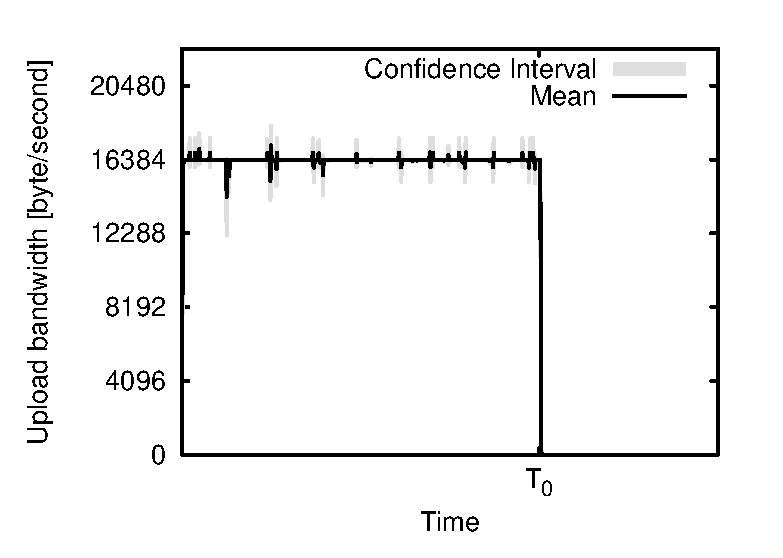
\includegraphics[width=0.49\textwidth]{fig/plots/scenario_16_chunk_count_fac_8/plots/GeneratedMeanCurrentSuperSeederUploadBandwidth.csv.eps}
  \end{center}
\end{frame}


%%%
%%% Szenario ChunkFac 16
%%%

\begin{frame}
  \frametitle{Default Szenario mit 16x Chunkanzahl - Completion}
  \begin{itemize}  
    \item Links: Ablauf des Datentransfers
    \item Rechts: Peers absteigend sortiert nach Gesamtdauer
  \end{itemize}

  \begin{center}
    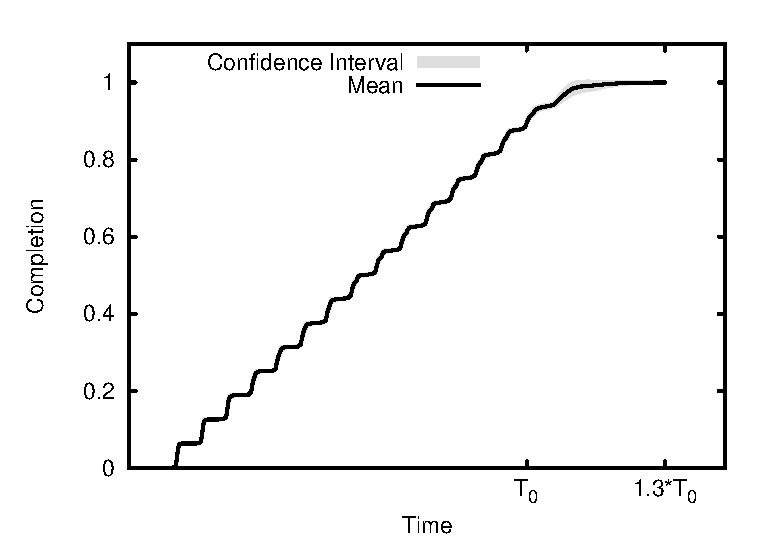
\includegraphics[width=0.49\textwidth]{fig/plots/scenario_17_chunk_count_fac_16/plots/GeneratedMeanChunkCompletion.csv.eps}
    \hfill
    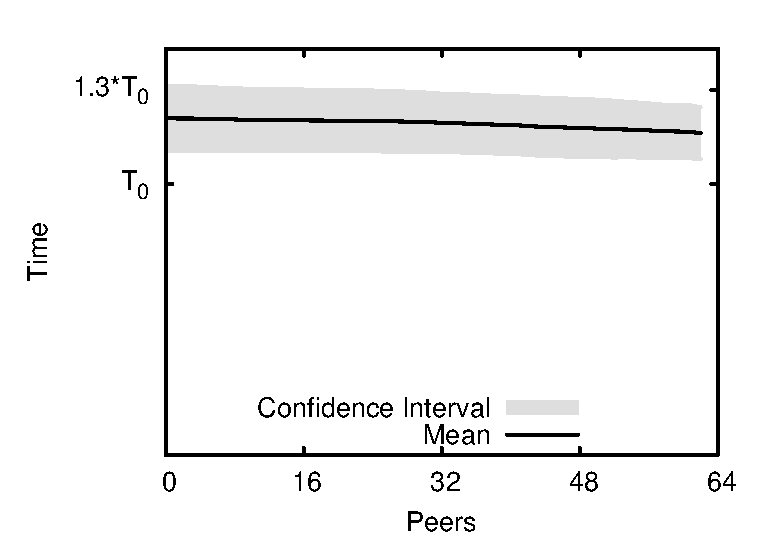
\includegraphics[width=0.49\textwidth]{fig/plots/scenario_17_chunk_count_fac_16/plots/GeneratedMeanSortedChunkCompletion.csv.eps}
  \end{center}
\end{frame}


\begin{frame}
  \frametitle{Default Szenario mit 16x Chunkanzahl - Upload/Download}
  \begin{center}
    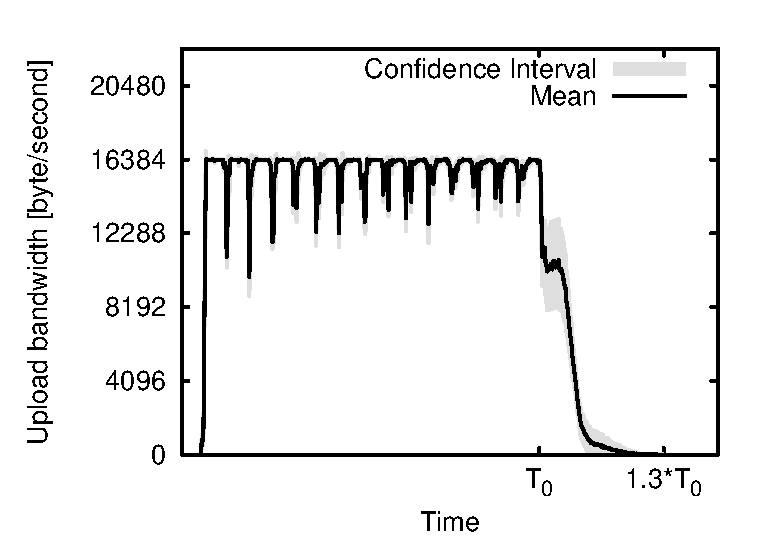
\includegraphics[width=0.49\textwidth]{fig/plots/scenario_17_chunk_count_fac_16/plots/GeneratedMeanCurrentUploadBandwidth.csv.eps}
    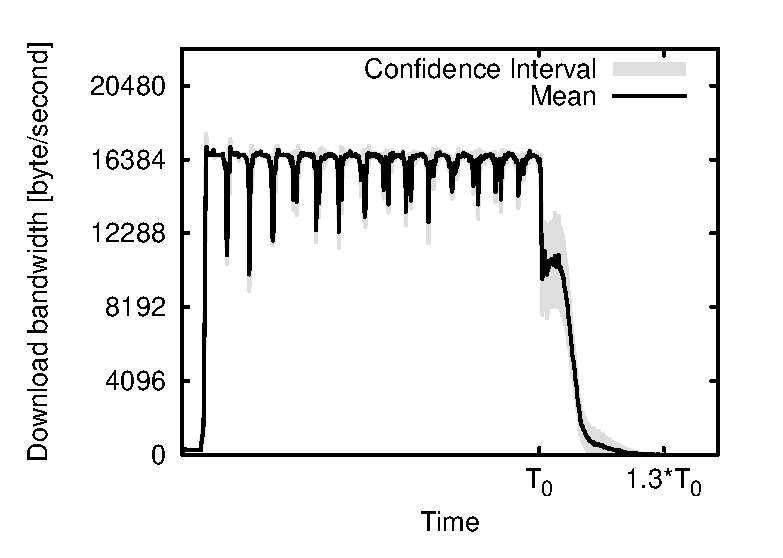
\includegraphics[width=0.49\textwidth]{fig/plots/scenario_17_chunk_count_fac_16/plots/GeneratedMeanCurrentDownloadBandwidth.csv.eps}
  \end{center}
\end{frame}


\begin{frame}
  \frametitle{Default Szenario mit 16x Chunkanzahl - Super-Peer Upload}
  \begin{center}
    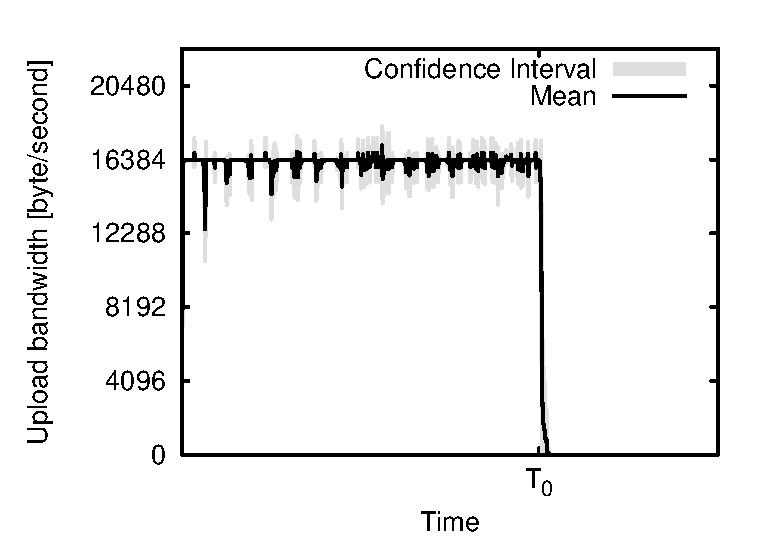
\includegraphics[width=0.49\textwidth]{fig/plots/scenario_17_chunk_count_fac_16/plots/GeneratedMeanCurrentSuperSeederUploadBandwidth.csv.eps}
  \end{center}
\end{frame}
